\documentclass[12pt]{article}

\usepackage{amsmath}
\usepackage{amsfonts}
\usepackage{amssymb}
\usepackage{graphicx}
\usepackage{float}
\usepackage{geometry}
\usepackage{subcaption}

\author{Benjamin Cox, Ricardo Velasco}
\title{Computer Modelling Exercise 3 Group Report}
\date{Due Thursday Week 11}

\begin{document}
	{\let\newpage\relax\maketitle}
	
	In this exercise we were tasked with implementing a class in python to represent a particle in three dimensions. We were to use that class and implement two different time integration algorithms (Euler and Verlet) and use these to simulate vibrating oxygen and nitrogen molecules. 
	
	One weakness of discrete integrators is their susceptibility to large errors when the timestep is set too large. Below are two plots with timesteps $\Delta t = 0.1u$ and $\Delta t = 1u$ over the same time interval. Each $u$ unit of time (for the timestep) corresponds to $10.8$fs.
	
	\begin{figure}[H]
		\centering
		\begin{subfigure}{0.45\textwidth}
			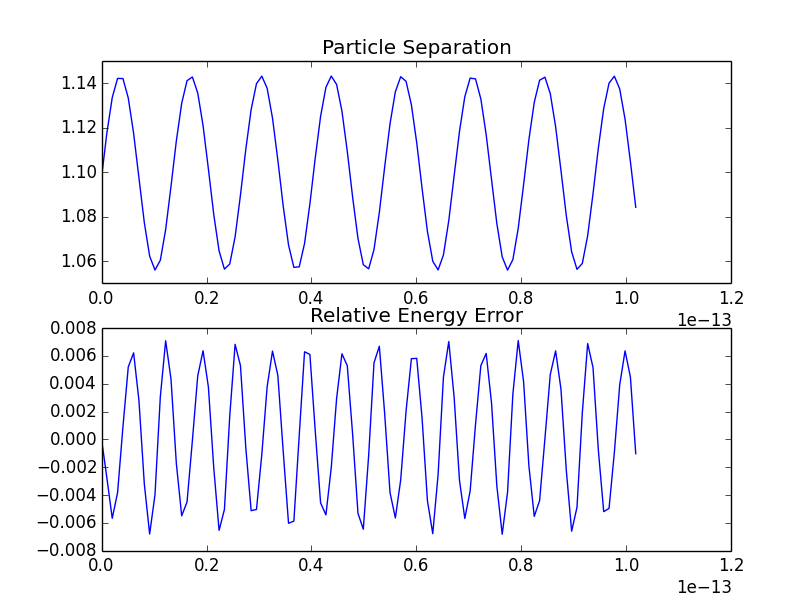
\includegraphics[width=\textwidth]{largedt}
			\caption*{$\Delta t = 0.1\times(10.8\text{fs})$}
		\end{subfigure}
		\begin{subfigure}{0.45\textwidth}
			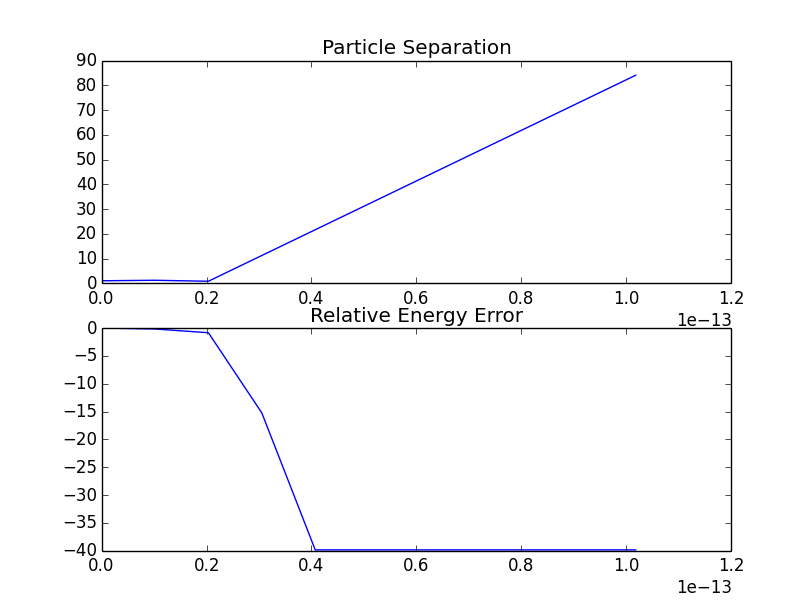
\includegraphics[width=\textwidth]{largerdt}
			\caption*{$\Delta t = 1\times(10.8\text{fs})$}
		\end{subfigure}
	\end{figure}
	
	The left figure is clearly showing signs of inaccuracy and is rather jagged. The right figure is wildly inaccurate.
	
	To determine the $dt_{\text{max}}$ we have to find the largest possible $dt$ such that the relative energy error has magnitude less than $10^{-3}$. This will be different for each integrator. For the velocity Verlet integrator we find that $dt_{\text{max}} \approx 0.1u $ For the symplectic Euler integrator we find that $dt_{\text{max}} \approx 0.015u,$ which is far smaller than the maximum timestep for the Verlet integrator. This shows that the Verlet integrator is more accurate with a larger timestep. 
	
When we run the Verlet integrator for a decent period of time with the timestep set to $dt_{\text{max}}$. We can determine the frequency of oscillation using XMGrace. We determine the period of $N_2$ without spin to be $T = 1.40\times 10^{-14}\text{s}$, so we determine $f = 1/T = 7.14\times 10^{13}\text{Hz}$ from which we derive the wavelength $\lambda$ using $c=\lambda f$. We see that $\lambda = 4.20\times10^{-6}m.$ To compute the inverse wavelength we take the inverse of this and see that $\nu(N_2) = 238260\text{m}^{-1}$ which corresponds to $\nu(N_2) = 2382\text{cm}^{-1}$ which is close to the experimental result of $\nu(N_2)= 2359cm^{-1}.$

Following the same procedure we will tabulate the vibrational frequencies below.

\begin{figure}[H]
\centering
\begin{tabular}{c|cc}
& Calculated Frequency (cm$^{-1}$) & Experimental Results (cm$^{-1}$)\\
\hline
$\nu(N_2)$ & & \\
No spin & 2382 & 2359\\
Spin & 2197 & --\\
\hline
$\nu(O_2)$ & & \\
No spin & 1564 & 1580 \\
Spin & 1506 & --\\
\end{tabular}
\end{figure}

The frequencies for the oscillation decrease for the systems in which the atoms have spin. This is because they are 

Below is a sample graph of the particle separations within the nitrogen with spin and the nitrogen without spin. 

	\begin{figure}[H]
		\centering
		\begin{subfigure}{0.45\textwidth}
			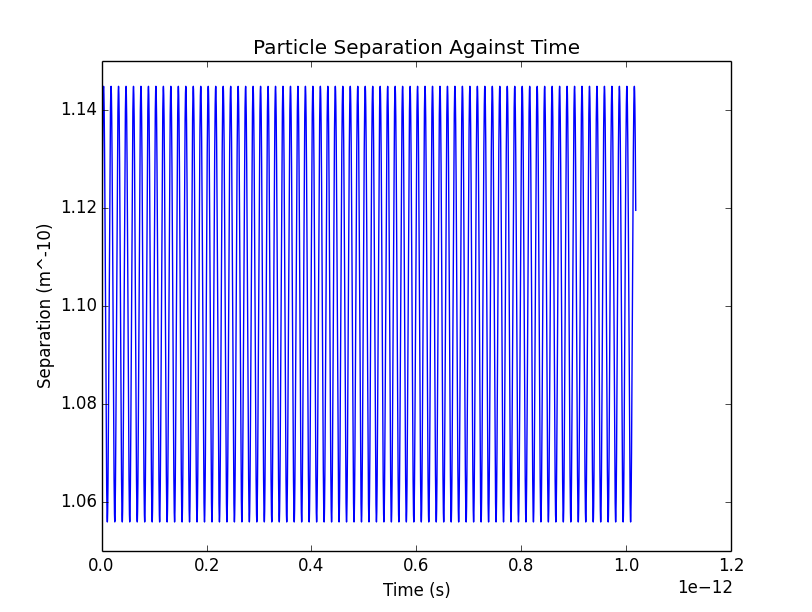
\includegraphics[width=\textwidth]{n2nospinsep}
			\caption*{$N_2$ particle separations without spin}
		\end{subfigure}
		\begin{subfigure}{0.45\textwidth}
			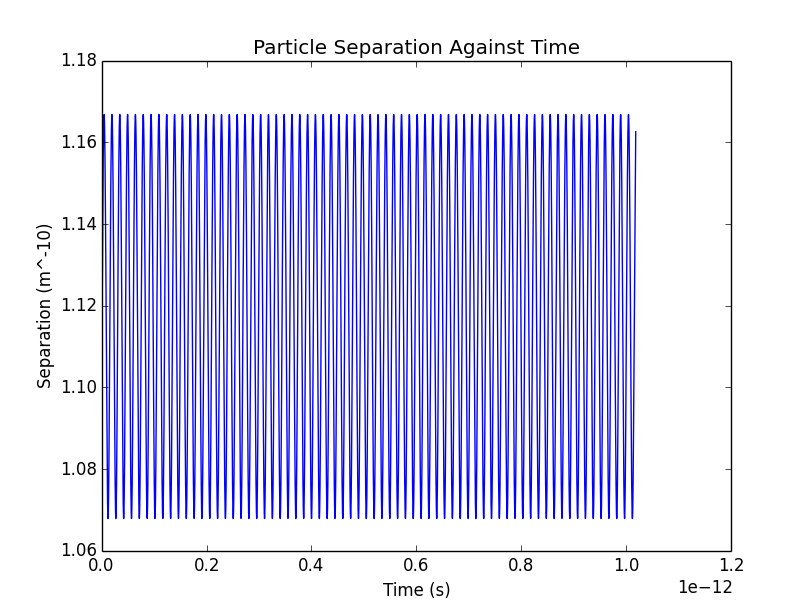
\includegraphics[width=\textwidth]{n2spinsep}
			\caption*{$N_2$ particle separations with spin}
		\end{subfigure}
	\end{figure}
	
It can be seen that the graphs look very similar on small scales such as these. However if you run them over a longer period of time you can see the difference in the envelope very clearly. 


	\begin{figure}[H]
		\centering
		\begin{subfigure}{0.45\textwidth}
			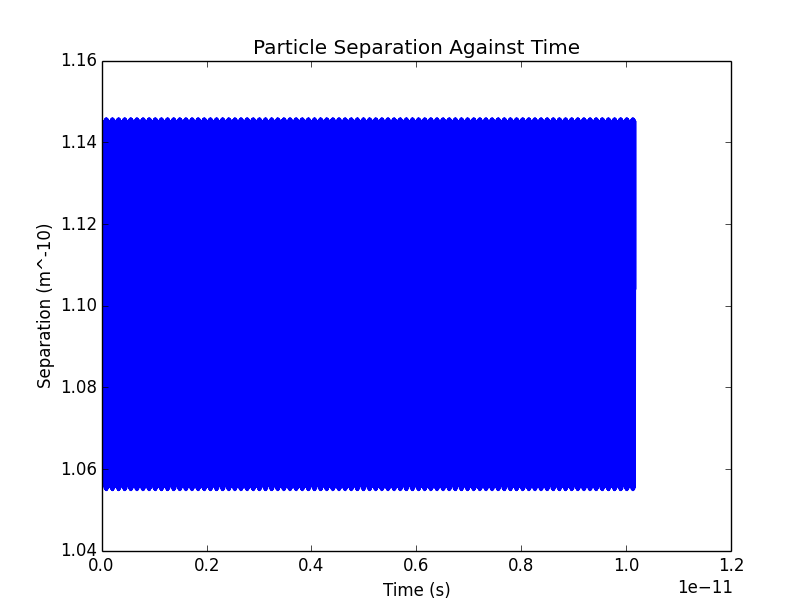
\includegraphics[width=\textwidth]{n2nospinlong}
			\caption*{$N_2$ particle separations without spin}
		\end{subfigure}
		\begin{subfigure}{0.45\textwidth}
			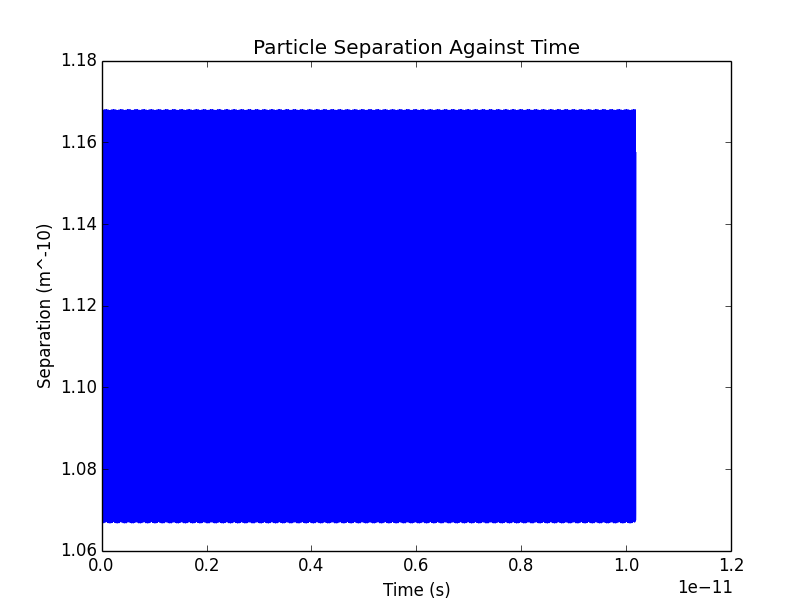
\includegraphics[width=\textwidth]{n2spinlong}
			\caption*{$N_2$ particle separations with spin}
		\end{subfigure}
	\end{figure}
	
You can see that the one without spin is more 'jagged', for lack of a better word.
The rest of the plots are contained at the end of the document.

Our results were close to the laboratory results but not exactly the same. They were slightly larger, likely due to the time integrator introducing error to the energy in the system. 

The velocity Verlet integrator performs better in both aspects; it performs better at a given timestep and has a larger maximum timestep. The symplectic Euler method would have caused our results to have far more error than they do if they were calculated at the same timestep. 

As it stands our results are within $\approx 1\%$ of the true value, meaning that a good amount of the error probably came from selecting and measuring the period. The integrator is accurate enough for our purposes, and definitely accurate enough to model the (non-relativistic) solar system. 

\pagebreak
\centering
	Graphs
	\begin{figure}[H]
		\centering
		\begin{subfigure}{0.45\textwidth}
			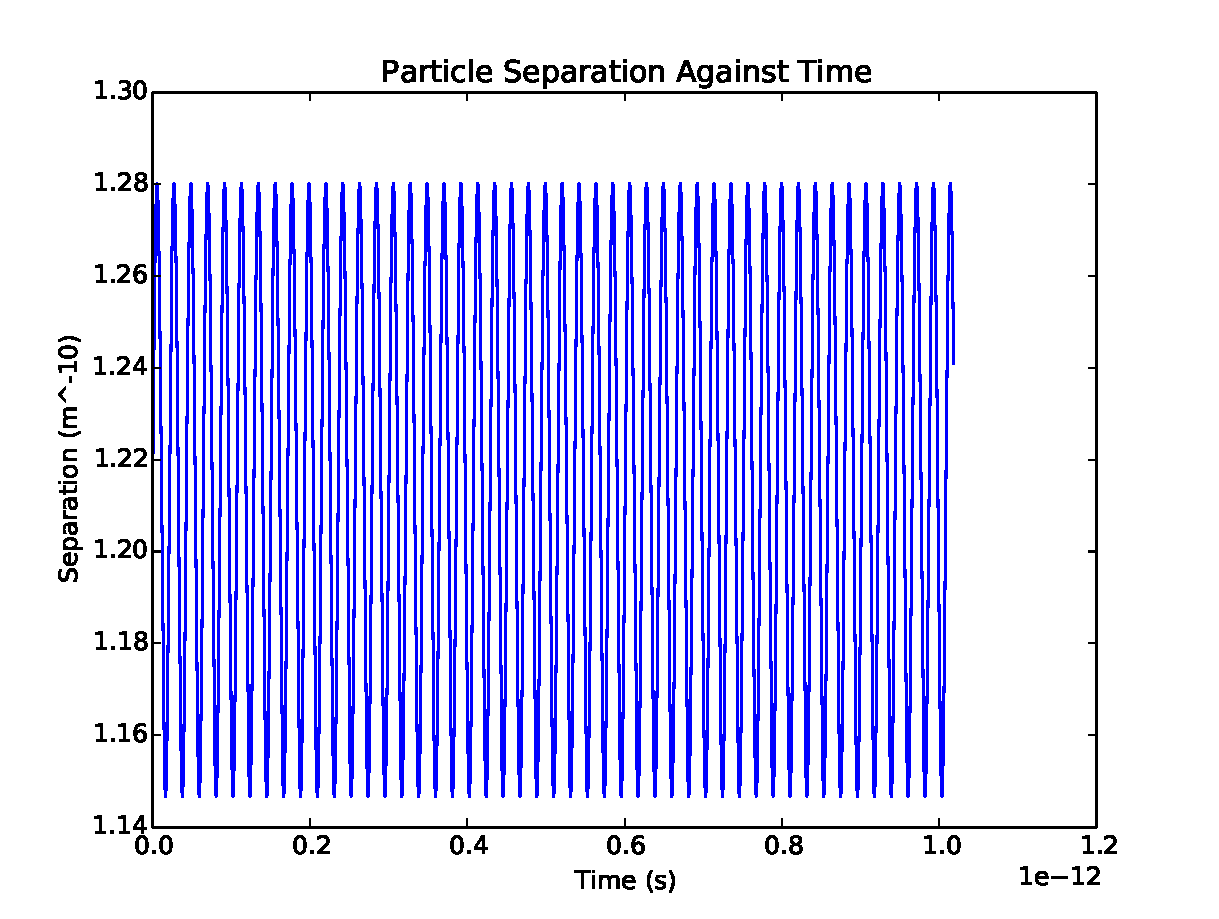
\includegraphics[width=\textwidth]{oxnospinshort}
			\caption*{$O_2$ particle separations without spin (short run)}
		\end{subfigure}
		\begin{subfigure}{0.45\textwidth}
			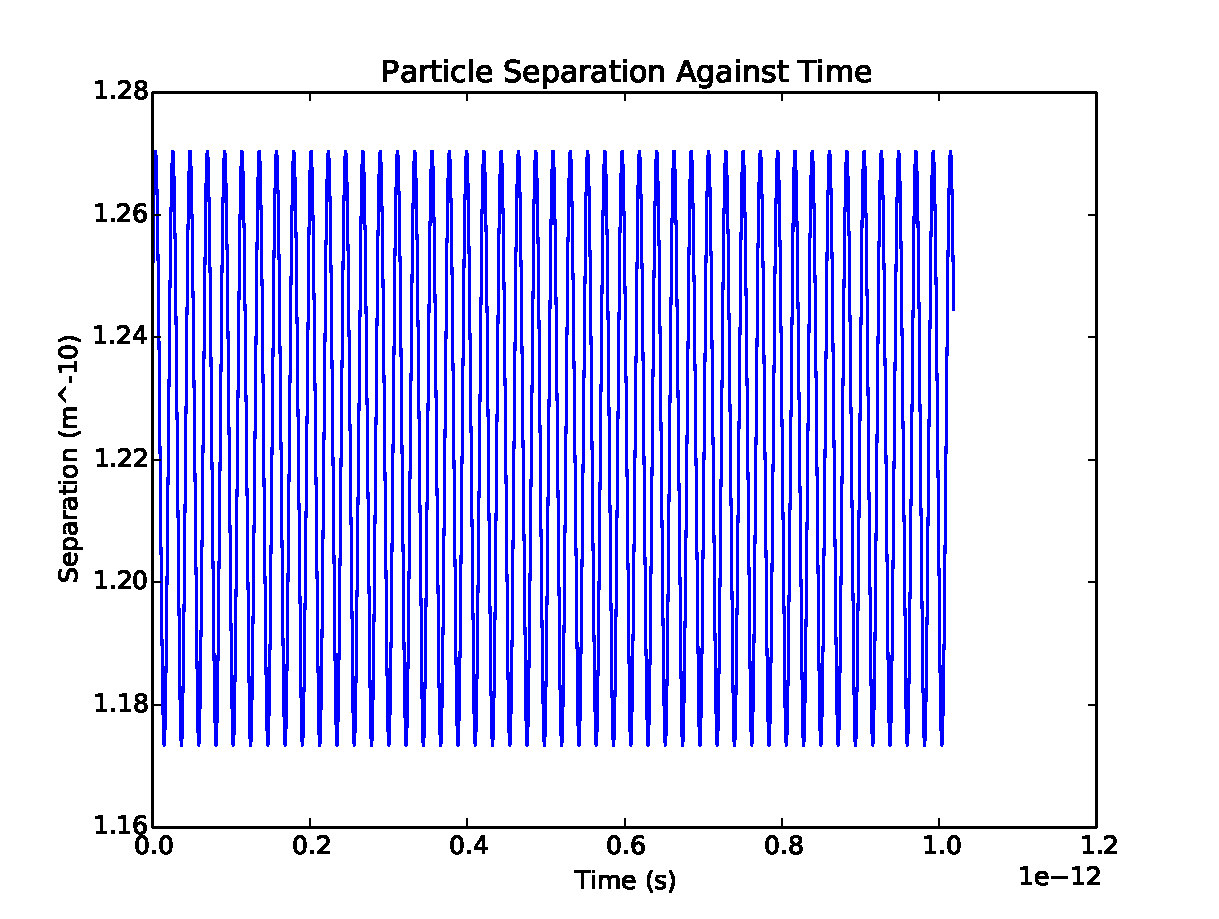
\includegraphics[width=\textwidth]{oxspinshort}
			\caption*{$O_2$ particle separations with spin (short run)}
		\end{subfigure}
	\end{figure}
	
	\begin{figure}[H]
		\centering
		\begin{subfigure}{0.45\textwidth}
			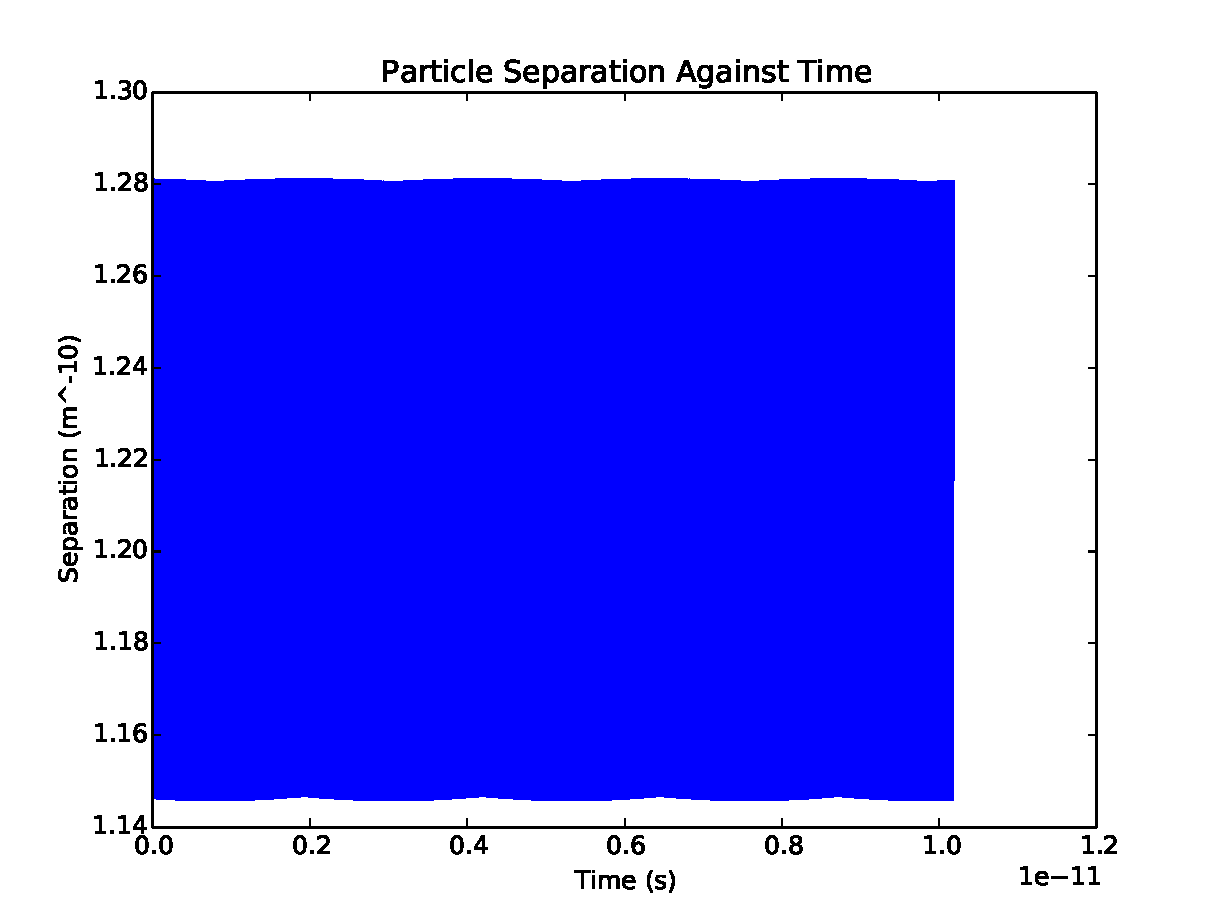
\includegraphics[width=\textwidth]{oxnospinlong}
			\caption*{$O_2$ particle separations without spin (long run)}
		\end{subfigure}
		\begin{subfigure}{0.45\textwidth}
			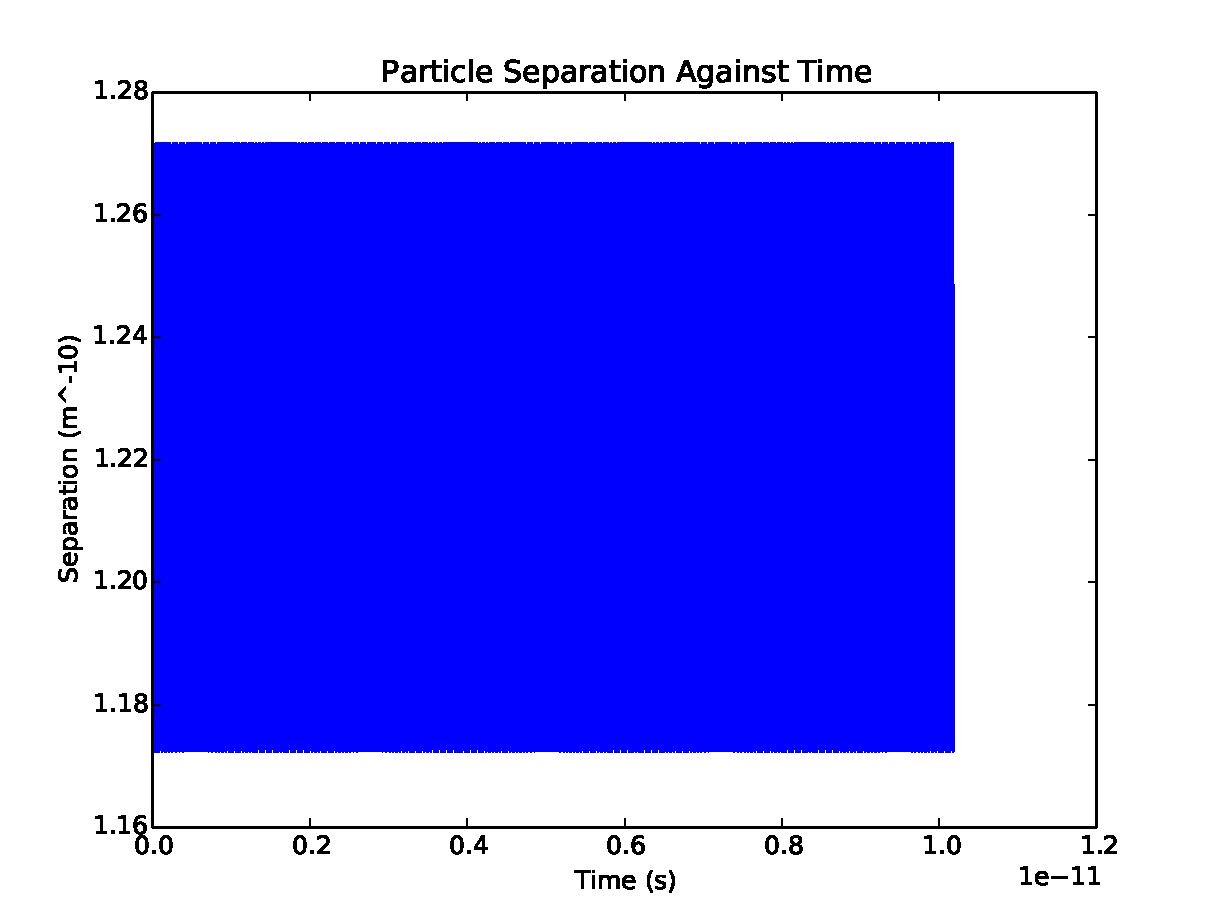
\includegraphics[width=\textwidth]{oxspinlong}
			\caption*{$O_2$ particle separations with spin (long run)}
		\end{subfigure}
	\end{figure}
	
	
\begin{figure}[H]
		\centering
		\begin{subfigure}{0.45\textwidth}
			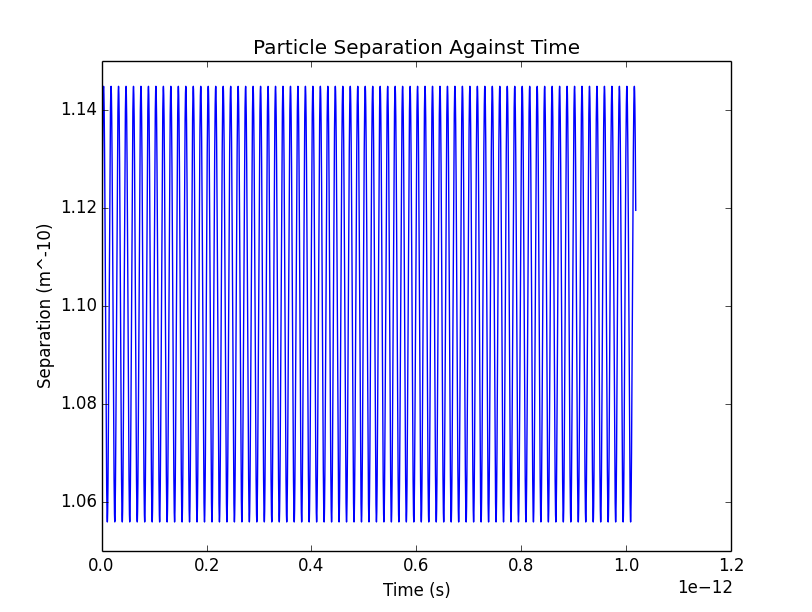
\includegraphics[width=\textwidth]{n2nospinsep}
			\caption*{$N_2$ particle separations without spin (short run)}
		\end{subfigure}
		\begin{subfigure}{0.45\textwidth}
			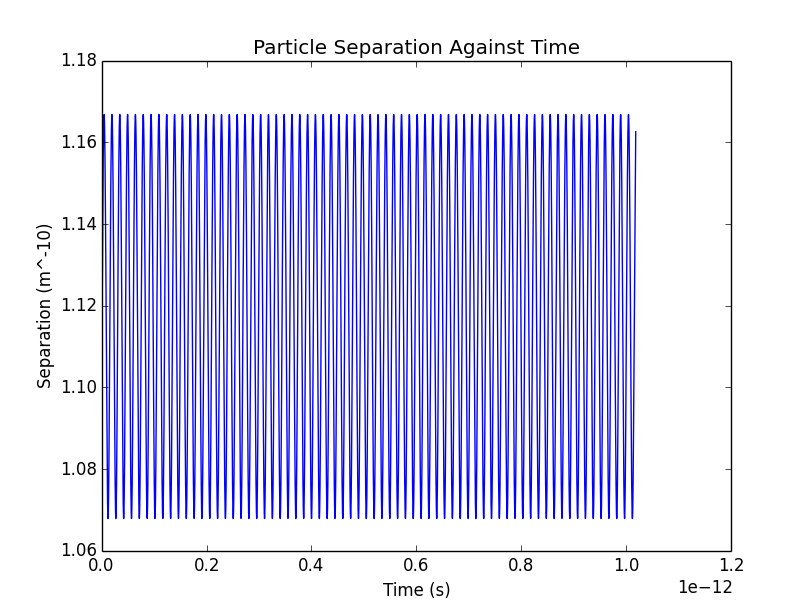
\includegraphics[width=\textwidth]{n2spinsep}
			\caption*{$N_2$ particle separations with spin (short run)}
		\end{subfigure}
	\end{figure}
	
	
\begin{figure}[H]
		\centering
		\begin{subfigure}{0.45\textwidth}
			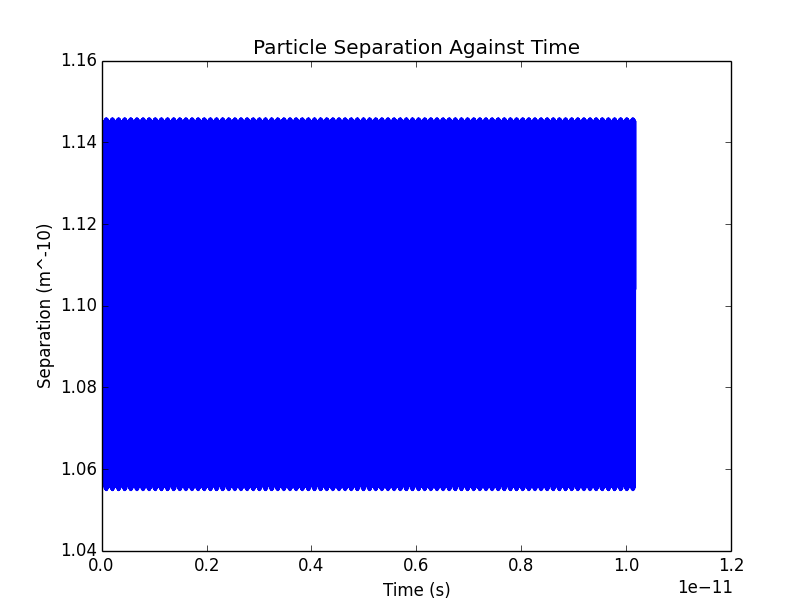
\includegraphics[width=\textwidth]{n2nospinlong}
			\caption*{$N_2$ particle separations without spin (long run)}
		\end{subfigure}
		\begin{subfigure}{0.45\textwidth}
			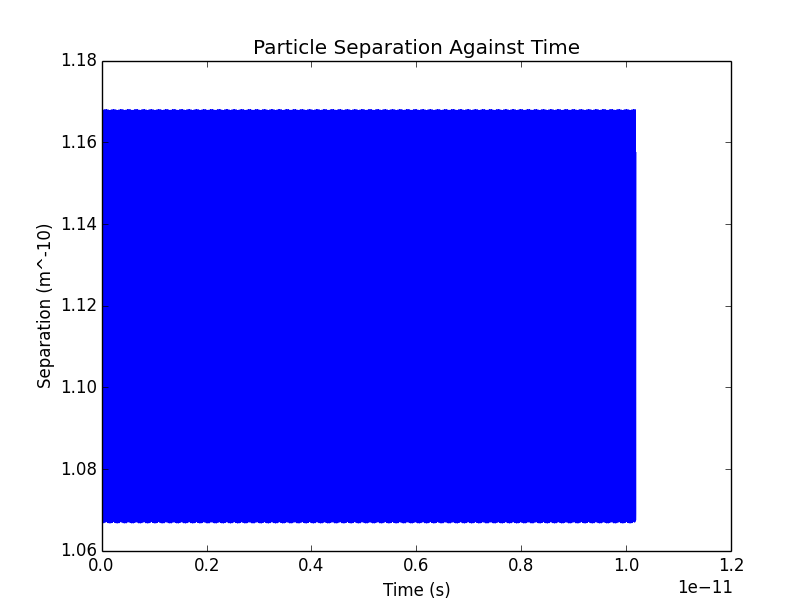
\includegraphics[width=\textwidth]{n2spinlong}
			\caption*{$N_2$ particle separations with spin (long run)}
		\end{subfigure}
	\end{figure}
\end{document}


